
%%% Local Variables: 
%%% mode: latex
%%% TeX-master: "report_dMRI_preprocessing.tex"
%%% End: 

\section{From raw data (DICOM format) to NIfTI format}
\label{sec:raw_to_nifti}
Digital Imaging and Communications in Medicine (DICOM) is the most common standard for receiving scans from a hospital. The DICOM standard was created by the National Electrical Manufacturers Association (NEMA) to aid the distribution and viewing of medical images, such as CT scans, MRIs, and ultrasound. A single DICOM file contains both a header (which stores information about the patient's name, the type of scan, image dimensions, etc), as well as all of the image data (which can contain information in three dimensions). 
\begin{figure} 
  \centering 
  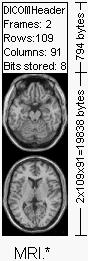
\includegraphics[width=66pt]{dicm1}
  \caption{An example of DICOM image file}
  \label{Fig:dicom_example}
\end{figure}

In figure \ref{Fig:dicom_example}, there is an example of the hypothetical DICOM image file. In this one, the first 794 bytes are used for a DICOM format header, which describes the image dimensions and retains other text information about the scan. The size of this header varies depending on how much header information is stored. Here, the header defines an image which has the dimensions 109x91x2 voxels, with a data resolution of 1 byte per voxel - so the total image size will be 19838. The image data follows the header information (the header and the image data are stored in the same file). More information about DICOM format can be found on the official webpage of DICOM~\footnote{\url{http://medical.nema.org/}}

Most of the MRI scanner produces T2-weighted DICOM data (.dcm). But DICOM data is quite complex leading to difficultly understanding. DICOM data needs to be converted in the format of NIfTI (Neuroimaging Informatics Technology Initiative). NIfTI is a modern incarnation of the Analyze format, but includes important information like the orientation of the image. It was for scientific analysis of brain images~\footnote{\url{http://nifti.nimh.nih.gov/}}. The format is simple, compact and versatile. The images can be stored as a pair of files (hdr/img, compliant with most Analyze format viewers), or a single file (nii). Many tools like FSL, NiBabel, MRIcron ... can also read compressed (nii.gz) images. One nice feature about NIfTI is that the format attempts to keep spatial orientation information. Therefore, NIfTI softwares that can read the spatial information should reduce your chance of making left-right errors. 

In this project, NiBabel is used to convert DICOM data to NIfTI. NiBabel is a pure python package~\footnote{\url{http://nipy.org/nibabel}}, and easy to run on any system. Result of this processing is NIfTI file image (.nii). NIFTI file image contains actual dMRI data (4D numpy.array, (I,J,K,W)), called \emph{native image}, and an\emph{affine}\footnote{\url{http://en.wikipedia.org/wiki/Affine_transformation}} transformation (2D, $4 \times 4$ numpy.array). The affine stores the information to map the volume i,j,k voxels in \emph{World coordinates}, which is a space in millimiter units. The world coordinate system, or \emph{native space}, is the coordinate system of the scanner.

\begin{figure} 
  \centering 
  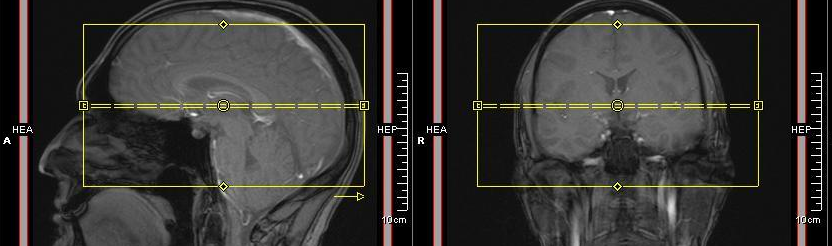
\includegraphics[width=14cm]{orthogonalrequire}
  \caption{Image acquired orthogonal to scanner bore}
  \label{Fig:orthogonal_require}
\end{figure}

Beside the NIfTI file image, most of DICOM image conversion tools also generate gradient vector (‘.bvec’) and b-value (‘.bval’) files. These files are very important to reconstruct diffusion properties. Because in diffusion tensor imaging (DTI) we construct tensors by collecting a series of direction-sensitive diffusion images. Therefore, in addition to recording the images, the scanner also saves these directions. A potential concern is that the scanner manufacturers can choose to either report the vectors with reference to the scanner bore, or with reference to the imaging plane (i.e., imaging grid). This is not a problem if the images are always acquired precisely orthogonal to the scanner bore (figure \ref{Fig:orthogonal_require}), as the image and scanner have the same frame of reference. However, problems can arise when the image plane is not aligned with the scanner bore (i.e., oblique acquisitions). In this situation, it is important to ensure that these vectors are in the same frame of reference as the image.Moreover, the eigenvectors of the tensor, and consequently tractography programs are sensitive to proper interpretation of the bvecs relative to the imaging plane.

Load NIfTI file image from memory
\begin{python}
nii_filename = < path_of_nifti_file_name >
img = nib.load(nii_filename)
\end{python}
Get data and affine transformation
\begin{python}
data = img.get_data()
affine = img.get_affine()
\end{python}
Get gradient vector (‘.bvec’) and b-value (‘.bval’) from files
\begin{python}
    bvec_filename = < path_of_bvec_file_name >
    bval_filename = < path_of_bval_file_name > 
    bvals = np.loadtxt(bval_filename)
    gradients = np.loadtxt(bvec_filename)
    assert(bvals.size==gradients.shape[0])
\end{python}

End of this step, all the necessary information for tracking have been extracted from the DICOM raw data including: actual dMRI data (4D numpy.array, (I,J,K,W)), affine transformation, gradient vector (‘.bvec’) and b-value (‘.bval’). In next stage, we will discuss how to create tractography from the actual dMRI data.
